\section{Der grundlegende Aufbau einer Android App}
Im nun folgenden Kapitel wird der grundlegende Aufbau einer Android App genauer beschrieben, wobei auf wichtige Bestandteile im Projekt eingegangen wird.
Zum einen soll hier der zugrundeliegende Dateiaufbau aber auch die Bestandteile einer App und deren Funktion genauer erl\"autert dargestellt werden. \cite{Android44}

\subsection{Componenten einer Applikation aus Sicht des Nutzers}
Eine App unter Android bestizt aus der sicht des Nutzers vier Hauptbestandteile:
\begin{itemize}
 \item Activity
 \item Broadcast Receiver
 \item Service
 \item ContentProvider
\end{itemize}

\subsubsection{Die Activity} \label{Die Activity aus Nutzersicht}
Eine Activity, unter Android, ist eine Benutzeroberfl\"ache in der App, wobei ein Projekt beliebig viele Activitys haben kann. Somit sind Activitys im eigentlichen Sinn Fenster, die in der Regel den gesamten Bildschirm f\"ullen und eine gewisse Aufgabe erf\"ullen. \cite{Kuehn12}

Der Aufruf verschiedener Activitys kann entweder vom Programmablauf vorgegeben sein oder durch Nutzeraktionen variieren. So kann zum Beispiel jenachdem welchen Button der Nutzer bet\"atigt eine andere Activity aufgerufen werden. \cite{Android44}

Eine Activity hat einen bestimmten Lebenszyklus den sie im Verlauf der Anwendung durchl\"auft. Beim erstellen einer Activity wird als erstes die Methode \texttt{onCreate} aufgerufen. Jenachdem welche Folgeaktion der Nutzer als n\"achstes ausf\"uhrt wird eine der Anderen Methoden wie im Bild \ref{ActivityLebenszyklus} aufgerufen. Wird die Activity wieder beendet, so wird die Methode \texttt{onDestroy} aufgerufen. 

Inaktiv ist eine Activity zum Beispiel dann, wenn die von einer anderen komplett oder Teilweise \"uberdeckt wird. Sollte eine neue Activity \"uber der alten ge\"offnet werden, wird diese nicht sofort zerst\"ort, sondern auf einer Art Stack gehalten von woaus sie wieder aufgerufen werden kann. Dies w\"are der Fall, wenn der Nutzer die Zur\"ucktaste bet\"atigt.

Activitys die sich im Stack befinden, werden erst gel\"oscht, wenn die zugeh\"orige App geschlossen oder Arbeitsspeicher freigegeben werden muss. 

Alle im Bild \ref{ActivityLebenszyklus} zu sehenden Methoden sind in der Tabelle \ref{Lebenszyklus-Methode einer Activity} im Kapitel \ref{Die Activity aus Programmierersicht} noch einmal genauer beschrieben.

\begin{figure}[!ht]
\centering
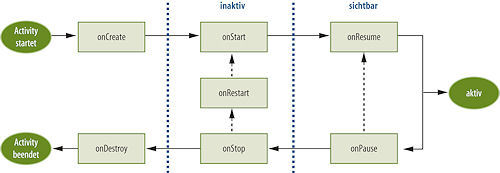
\includegraphics[width=12cm]{Bilder/ActivityLifecycle}
\caption{Der Lebenszyklus einer Activity \cite{ActivityLifecycle}}
\label{ActivityLebenszyklus}
\centering
\end{figure}
\FloatBarrier

% In der folgenden Tabelle sind alle m\"oglichen Methoden beschrieben, welche im Lebenszyklus einer Activity vom Betriebssystem aufgerufen werden k\"onnen.

\subsubsection{Broadcast Receiver} \label{Broadcast Receiver aus Nutzersicht}
Ein Broadcast Receiver unter Android ist ein Empf\"anger f\"ur verschiedene Benachrichtigungen die vom Betriebssystem abgesetzt werden. Benachrichtigungen unter Android sind vielf\"altig und k\"onnen zum Beispiel bei erhalt einer SMS oder E-Mail gesendet werden. Alle im System registrieten Receiver werden bei ihrem zugeh\"origen Event aktiv und bleiben dies auch nur f\"ur die Zeit, welche es ben\"otigt die Methode \texttt{onReceive} auszuf\"uhren.

Android unterscheidet grunds\"atzlich zwei verschiedene Arten von Broadcast Receivern und zwar Dynamische und Statische Broadcast Receiver. Dynamische Broadcast Receiver sind nicht im System registriert und k\"onnen nur zur Laufzeit der Komponente (Activity oder Service) auf Ereignisse reagieren. Statische Broadcast Receiver hingegen m\"ussen im Betriebssystem registriert werden. Hierf\"ur m\"ussen sie in der Manifest-Datei deklariert sein, wie eine Manifest-Datei aufgebaut ist, ist im Kapitel \ref{Die Manifest-Datei} genauer beschrieben. Durch die Regisitrierung im System muss die zugeh\"orige App nicht laufen um einen Broadcast zu empfangen und zu verarbeiten.

\subsubsection{Services} \label{Services aus Nutzersicht}
Services in Android sind gedacht f\"ur Programmbestandteile, welche keine Benutzeroberfl\"ache ben\"otigen. Hintergrundprozesse, wie zum Beispiel das abspielen von Musik oder das herunterladen von Daten sind typische Anwendungsf\"alle f\"ur Services. 

Wie schon bei den Broadcast Receivern gibt es im Androidsystem zwei Arten von Services, zum einen den Loacl Service welcher an eine bestimmte Komponente gebunden ist und zum anderen Remote Services, welche in einem eigenen Prozess laufen auch nachem die App beendet wurde.

\subsubsection{ContentProvider}

\subsection{Componenten einer Applikation aus Sicht des Programmierers}
Eine App besteht f\"ur den Programmierer nat\"urlich aus sehr viel mehr als nur die vier f\"ur den Nutzer sichtbaren Teile. Welche das sind und welche Aufgaben sie haben ist im folgenden genauer beschrieben.

\subsubsection{Die Manifest-Datei} \label{Die Manifest-Datei}
Das Android Manifest ist die Schaltzentrale einer App, in der alle Bestandteile einer Applikation aufgef\"uhrt sind. Das Manifestunter Android ist also XML-Datei im Wurzelverzeichnis abgelegt. 

Im Manifest sind als erstes Informationen zum Package-Name zu sehen (1) welche direkt vor der Versionsnummer und dem Versionsnamen zufinden sind (2). Unter \texttt{uses-sdk} ist zum einen die Angabe zur minimalen Android-Version angegeben und zum anderen mit welcher Version Kompiliert wurde (3). \texttt{uses-permission} gibt an, welche Berechtigungen die App in anspruch nimmt (4). Zum Schluss m\"ussen nat\"urlich auch noch alle Activitys und Services angegeben werden (5).
\cite{Android44}

Im Listing ist eine Manifest-Datei beispielhaft zu sehen.

\lstinputlisting{Code/ManifestExample.xml}

\subsubsection{Intents} \label{Intents}

\subsubsection{Die Activity} \label{Die Activity aus Programmierersicht}
Activitys sind wie im Kapitel \ref{Die Activity aus Nutzersicht} schon dargestellt die Benutzeroberfl\"ache, welche der Nutzer sieht, und mit der er Interagieren kann.

Eine Activity-Klasse erbt von der Android-API-Klasse \texttt{ActionBarActivity} und hat die in der Tabelle \ref{Lebenszyklus-Methode einer Activity} aufgef\"uhrten wichtigen Methoden, welche sie von der Oberklasse erbt.

% \FloatBarrier
\begin{table}[!ht]
\begin{tabular}{|p{3cm}|p{12cm}|}
 \hline Methode & Beschreibung \\
 \hline onCreate & Diese Methode wird beim erzeugen der Activity aufgerufen und kann wie ein Konstruktor verwendet werden. Es werden alle Felder, Formulare, Men\"us und Layouts hier initialisiert.\\&\\
 onStart & Wird ausgef\"uhrt, wenn die Activity neu erzeugt wird oder sie aus dem Hintergrund wieder hervortritt, wie es zum Beispiel beim dr\"ucken der Zur\"ucktaste der Fall ist.\\&\\
 onResume & Wenn eine teilweise verdeckte Activity wieder in den Focus r\"uckt wird diese Methode Aufgerufen.\\&\\
 onPause & Diese Methode wird Ausgef\"uhrt, wenn die Activity teilweise verdeckt wird und somit inaktiv wird.\\&\\
 onStop & Wird ausgef\"uhrt, wenn die Activity in den Hintergrund tritt und auf den Stack abgelegt wird.\\&\\
 onRestart & Die Activity r\"uckt vom Stack wieder in den Vordergrund weil diese wieder ben\"otigt wird.\\&\\
 onDestroy & Diese Methode wird ausgef\"uhrt, wenn die Activity beendet wird. In ihr sollten alle belegten Ressourcen wieder freigegeben werden.\\
 \hline
\end{tabular}
\caption{Lebenszyklus-Methode einer Activity \cite{Android44}}
\label{Lebenszyklus-Methode einer Activity}
\end{table}
\FloatBarrier

\subsubsection{Broadcast Receiver} \label{Broadcast Receiver aus Programmierersicht}
Eine Broadcast-Receiver-Klasse erbt von der Android-API-Klasse \texttt{BroadcastReceiver}. Ein Broadcast Receiver erbt nur die Methode \texttt{onReceive} welche Ausgef\"uhrt wird, wenn ein Broadcast empfangen wird. Hieraus wird auch ersichtlich, das ein Broadcast Receiver nur zur Zeit der Ausf\"uhrung existiert.

Um einen Statischen Receiver im Manifest einzutragen wird ein Eintrag in der Manifest-Datei ben\"otigt, wie im Listing unten beispielhaft f\"ur einen Receiver der auf das Event \texttt{BOOT\_COMPLETED} reagiert dargestellt ist. Dieser Receiver wird ausgef\"uhrt, wenn das System fertig gebootet hat. Zum einen wird der Name der Receiver-Klasse eingetragen (BootReceiver), zum anderen auf welchen Intent er reagieren soll (im Beispiel \texttt{BOOT\_COMPLETED}).

\lstinputlisting{Code/BroadcastReceiverManifest.xml}

Ein Dynamischer Broadcast Receiver wird einfach innerhalb einer Javaklasse zum Beispiel einer Activity aufgerufen und ist dann f\"ur die Lebensdauer der Komponente aktiv. Wird die Komponente geschlossen kann der Receiver folglich nicht mehr reagieren.

\subsubsection{Services} \label{Services}
Wie schon im Kapitel \ref{Services aus Nutzersicht} vorgestellt, gibt es unter Android die Local Services und die Remote Services. Beide Arten m\"ussen in der Manifest-Datei aufgef\"uhrt werden, wobei ein Local Servie nur mit dem Klassenname angegeben werden muss, wie das Listing zeigt. Der Klassenname des Service ist im Beispiel "`DatabaseService"', der Punkt sagt aus, dass sich die Klasse im selben Verzeichnis wie das Manifest befindet.

\lstinputlisting{Code/LocalServiceManifest.xml}

Ein Remote Service ben\"otigt zus\"atzlich zum Klassennamen noch einen Prozessnamen, da der Service ja in einem eigenen Prozess starten soll. Das Listig vom Local Service muss also im den Prozessnamen erweitert werden.

Der Doppelpunkt vor dem Namen (im Listing "`MyDatabaseService"') sagt aus, dass der Service in einem eigenen Prozess starten soll.

Sollte der Servicename mit einem Gro\ss{}buchstaben beginnen, so l\"auft er unter dem selben User wie die App selbst und kann somit nur von der App angesprochen werden, da wie im Kapitel \ref{Das Sandbox Prinzip} beschrieben jede App unter einem anderen User l\"auft. Beginnt der Servicename jedoch mit einem Kleinbuchstaben so l\"auft er global und kann von jeder App angesprochen werden.

\lstinputlisting{Code/RemoteServiceManifest.xml}

Ein Local Service wird mit der Methode \texttt{startService} gestartet und besitzt die folgenden Lebenszyklus-Methoden wie sie in der Tabelle \ref{Lebenszyklus-Methode eines Local Service} aufgef\"uhrt sind.

% \FloatBarrier
\begin{table}[!ht]
\begin{tabular}{|p{3cm}|p{12cm}|}
 \hline Methode & Beschreibung \\
 \hline onCreate & Diese Methode wird beim erzeugen des Service  und kann wie ein Konstruktor verwendet werden. Sie sollte f\"ur Initialisierungen genutzt werden.\\&\\
 onStartCommand & Wird aufgerufen, wenn die Methode \"uber \texttt{Context.startService} gestartet wird und ist neu seit Android 2.0.\\&\\
 onDestroy & Diese Methode wird aufgerufen, wenn der Service beendet wird, wobei ein Service sich auch \"uber die Methode \texttt{stopSelf} selbstst\"andig beenden kann.\\
 \hline
\end{tabular}
\caption{Lebenszyklus-Methode eines Local Service \cite{Android44}}
\label{Lebenszyklus-Methode eines Local Service}
\end{table}
\FloatBarrier

Ein Remote Service wird an eine Activity gebunden und wird \"uber die Methode \texttt{bindService} gestartet. In der Tabelle \ref{Lebenszyklus-Methode eines Remote Service} sind die Lebenszyklus-Methoden eines Remote Services.

\FloatBarrier
\begin{table}[!ht]
\begin{tabular}{|p{3cm}|p{12cm}|}
 \hline Methode & Beschreibung \\
 \hline onCreate & Wie in Tabelle \ref{Lebenszyklus-Methode eines Local Service}.\\&\\
 onBinde & Wird aufgerufen, sobald sich eine Komponente mit dem Service Verbindet und gibt eine Instanz vom Typ \texttt{IBinder} zur\"uck.\\&\\
 onUnbinde & Wird aufgerufen, wenn die Komponente die Verbindung zum Service beendet.\\&\\
 onDestroy & Wie in Tabelle \ref{Lebenszyklus-Methode eines Local Service}.\\
 \hline
\end{tabular}
\caption{Lebenszyklus-Methode eines Remote Service \cite{Android44}}
\label{Lebenszyklus-Methode eines Remote Service}
\end{table}
\FloatBarrier

\subsubsection{ContentProvider}